% Source-faithful schematic draft: 2006 Chongqing Science Q19, PDF p.2 (printed p.285).
% Source ID: src-5abd831561d7d4fa968c5bf0deb634e0d666376fd8cc90967cf30d301e77a351
% Source SHA-256: 211d79b8676187c7e4a98c71d7eae5eadd28b2e5aaf9237fefd55a791241faa3
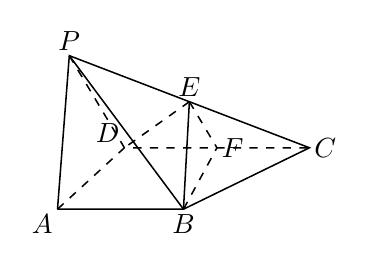
\begin{tikzpicture}[line width=0.55pt,every node/.style={inner sep=1.5pt}]
 % The base is shown in oblique projection; dashed segments reproduce hidden edges in the source.
 \coordinate (A) at (0,0); \coordinate (B) at (1.6,0); \coordinate (D) at (0.85,0.78); \coordinate (C) at (3.2,0.78); \coordinate (P) at (0.15,1.95);
 \coordinate (E) at (1.675,1.365); % E is the projected midpoint of PC
 \coordinate (F) at (2.025,0.78); % midpoint of CD in the drawn projection
 \draw (A)--(B)--(C)--(P)--(A);
 \draw (P)--(B);
 \draw[dashed] (A)--(D)--(C);
 \draw[dashed] (P)--(D);
 \draw (E)--(B);
 \draw[dashed] (E)--(D) (E)--(F) (B)--(F);
 \foreach \pt/\pos/\lab in {A/below left/A,B/below/B,C/right/C,D/above left/D,P/above/P,E/above/E,F/right/F}
   \node[\pos] at (\pt) {$\lab$};
\end{tikzpicture}
